%%% CSE 4317 DDS - WORKED EXAMPLE (Computer Vision / ML). Follows IEEE Std 1016-2009.
\documentclass[11pt,letterpaper]{article}
\usepackage[margin=1.0in]{geometry}
\usepackage[T1]{fontenc}\usepackage[bitstream-charter]{mathdesign}\usepackage[latin1]{inputenc}
\usepackage{amsmath}\usepackage{xcolor}\usepackage{cite}\usepackage{hyphenat}
\usepackage{graphicx}\usepackage{float}\usepackage{subfigure}\usepackage{sectsty}
\usepackage[compact]{titlesec}\usepackage[tablegrid]{vhistory}\usepackage{pbox}\usepackage{longtable}
\usepackage{tikz}\usetikzlibrary{positioning,arrows.meta,fit,backgrounds}
\allsectionsfont{\color{accentcolor}\scshape\selectfont}
\definecolor{accentcolor}{rgb}{0.0,0.0,0.5}
\tikzset{
  mod/.style={draw, rounded corners, fill=white, minimum height=8mm, minimum width=27mm, font=\footnotesize, align=center, inner sep=2pt},
  ext/.style={draw, dashed, rounded corners, fill=black!4, minimum height=8mm, minimum width=24mm, font=\footnotesize\itshape, align=center, inner sep=2pt},
  band/.style={draw=accentcolor!45, rounded corners, inner sep=3.5mm},
  llbl/.style={font=\small\bfseries, text=accentcolor, align=left},
  flow/.style={-{Latex[length=2mm]}, thick, draw=accentcolor!80},
  fl/.style={font=\scriptsize, fill=white, inner sep=1pt},
}
\newcommand{\teamname}{Team Perceptron}
\newcommand{\productname}{DigitDesk Handwritten Form Digitization Service}
\newcommand{\coursename}{CSE 4317: Senior Design II}
\newcommand{\semester}{Spring 2027}
\newcommand{\docname}{Detailed Design Specification}
\newcommand{\department}{Department of Computer Science \& Engineering}
\newcommand{\university}{The University of Texas at Arlington}
\newcommand{\authors}{Alan Turing \\ Grace Hopper \\ John Von Neumann \\ Ada Lovelace \\ Charles Babbage}
\usepackage{fancyhdr}\pagestyle{fancy}\usepackage{lastpage}
\lhead{}\chead{}\rhead{}\lfoot{\footnotesize \teamname \ - \semester}\cfoot{}
\rfoot{\footnotesize page \thepage\ of \pageref{LastPage}}
\renewcommand{\headrulewidth}{0.0pt}\renewcommand{\footrulewidth}{0.4pt}
\usepackage[runin]{abstract}\abslabeldelim{\quad}\setlength{\abstitleskip}{-10pt}
\renewcommand{\abstractname}{}\renewcommand{\abstracttextfont}{\color{accentcolor} \small \slshape}

\begin{document}
{\centering \huge \color{accentcolor} \sc \textbf{\department \\ \university} \par}
\vspace{1 in}
{\centering \huge \color{accentcolor} \sc \textbf{\docname \\ \coursename \\ \semester} \par}
\vspace{0.5 in}
\begin{figure}[h!]\centering
\includegraphics[width=0.60\textwidth]{images/test_image}\end{figure}
\vspace{0.5 in}
{\centering \huge \color{accentcolor} \sc \textbf{\teamname \\ \productname} \par}
\vspace{0.5 in}{\centering \large \sc \textbf{\authors} \par}
\newpage
\begin{versionhistory}
  \vhEntry{0.1}{01.20.2027}{AL}{document creation}
  \vhEntry{1.0}{02.05.2027}{AT|GH|CB}{official release}
\end{versionhistory}
\newpage\setcounter{tocdepth}{2}\tableofcontents\newpage

\section{Introduction}
Implementation-level design of \productname\ as an IEEE 1016-2009 \cite{IEEE1016}
Software Design Description, building on the SRS and ADS (layers X/Y/Z).

\section{Design Stakeholders \& Concerns}
Implementers, integrators, testers, maintainers; concerns of composition, data,
interfaces, algorithms, state, and resources.

\section{Design Viewpoints}
Context, Composition, Information, Interface, Interaction \& State, Algorithm, and
Resource viewpoints per IEEE 1016; irrelevant viewpoints omitted per subsystem.

\section{System Overview}
\begin{figure}[h!]\centering\resizebox{\textwidth}{!}{%
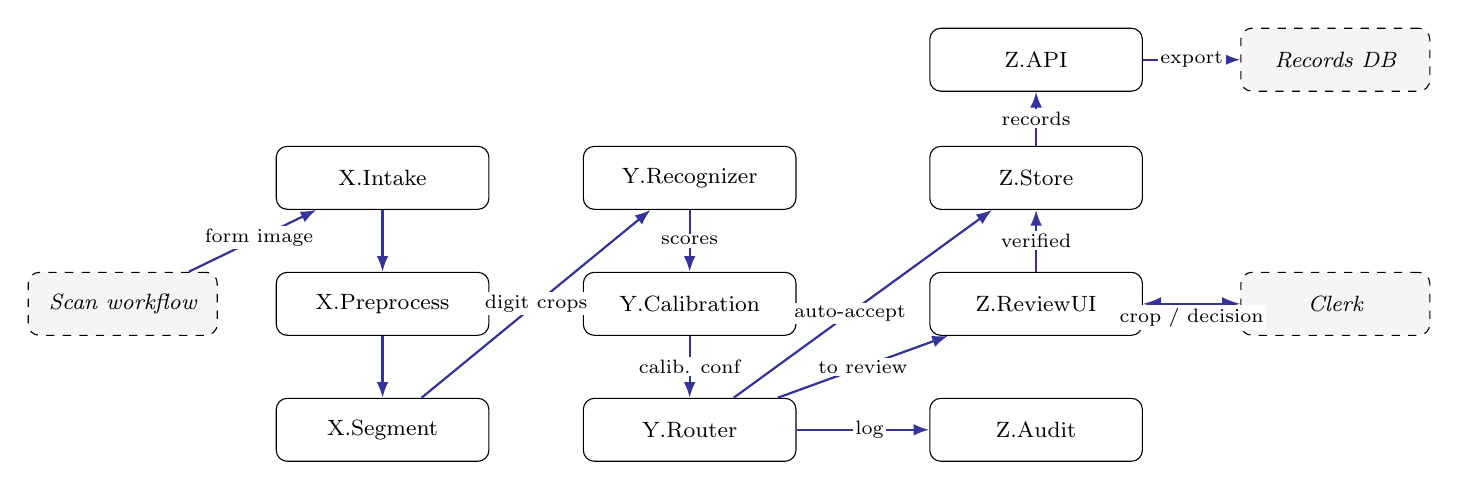
\begin{tikzpicture}
\node[ext] (scan) at (0,0) {Scan workflow};
\node[mod] (xin)  at (3.3,1.6) {X.Intake};
\node[mod] (xpre) at (3.3,0)   {X.Preprocess};
\node[mod] (xseg) at (3.3,-1.6){X.Segment};
\node[mod] (yrec) at (7.2,1.6) {Y.Recognizer};
\node[mod] (ycal) at (7.2,0)   {Y.Calibration};
\node[mod] (yrou) at (7.2,-1.6){Y.Router};
\node[mod] (zapi) at (11.6,3.1){Z.API};
\node[mod] (zsto) at (11.6,1.6){Z.Store};
\node[mod] (zrev) at (11.6,0)  {Z.ReviewUI};
\node[mod] (zaud) at (11.6,-1.6){Z.Audit};
\node[ext] (clerk) at (15.4,0) {Clerk};
\node[ext] (recdb) at (15.4,3.1){Records DB};
\draw[flow] (scan) -- (xin) node[fl,pos=0.55]{form image};
\draw[flow] (xin) -- (xpre);
\draw[flow] (xpre) -- (xseg);
\draw[flow] (xseg) -- (yrec) node[fl,pos=0.5]{digit crops};
\draw[flow] (yrec) -- (ycal) node[fl,pos=0.5]{scores};
\draw[flow] (ycal) -- (yrou) node[fl,pos=0.5]{calib. conf};
\draw[flow] (yrou) -- (zsto) node[fl,pos=0.45]{auto-accept};
\draw[flow] (yrou) -- (zrev) node[fl,pos=0.5]{to review};
\draw[flow] (yrou) -- (zaud) node[fl,pos=0.55]{log};
\draw[{Latex}-{Latex}, thick, draw=accentcolor!80] (zrev) -- (clerk) node[fl,pos=0.5,below]{crop / decision};
\draw[flow] (zrev) -- (zsto) node[fl,pos=0.5]{verified};
\draw[flow] (zsto) -- (zapi) node[fl,pos=0.5]{records};
\draw[flow] (zapi) -- (recdb) node[fl,pos=0.5]{export};
\end{tikzpicture}}
\caption{Pipeline carried forward from the ADS}\end{figure}
Deployed as Docker containers on an on-prem Linux host with a message queue
(RabbitMQ) between stages and PostgreSQL + object storage for persistence.

\section{X Layer Subsystems --- Ingestion \& Preprocessing}
\subsection{Layer Resources}
\textbf{OS/Deps:} Linux, Python, OpenCV, Pillow; \textbf{Language:} Python.
\subsection{X.Segment}
\textbf{Composition:} a worker consuming preprocessed pages.
\textbf{Information:} \texttt{Field\{form\_id, field\_id, bbox, crop[]\}}.
\textbf{Interface (\#01 chain):} in preprocessed page; out field crops to queue.
\textbf{Algorithm:} affine-align the page to the template via fiducial marks, then
crop fixed field boxes; reject pages whose alignment residual exceeds a threshold.
\textbf{Rationale:} deterministic and testable for a fixed template (AD-01).

\section{Y Layer Subsystems --- Recognition \& Analytics}
\subsection{Layer Resources}
\textbf{Deps:} PyTorch, NumPy; \textbf{Language:} Python; GPU optional.
\subsection{Y.Recognizer}
\textbf{Information:} input \texttt{Field}; output
\texttt{Prediction\{value, logits[], model\_version, data\_hash\}} (MS-01).
\textbf{Interface (\#02):} in field crops; out predictions.
\textbf{Algorithm:} a small CNN (LeNet/MobileNet-class) over per-digit crops; the
field value is the ordered concatenation of per-digit argmax. \textbf{Resource:}
model artifact loaded from a versioned path (QA-01).
\subsection{Y.Calibration \& Y.Router}
\textbf{Y.Calibration:} temperature-scaled softmax fit on a held-out set converts
logits to a calibrated field confidence. \textbf{Y.Router:} \texttt{if conf $\geq$
threshold: accept else: enqueue\_review} (FR-03); threshold in config.

\section{Z Layer Subsystems --- Service, Storage \& Review}
\subsection{Layer Resources}
\textbf{Deps:} FastAPI, PostgreSQL, React (review UI); \textbf{Languages:} Python,
TypeScript.
\subsection{Z.API \& Z.Store}
\textbf{Interface:} \texttt{POST /forms} (EI-01), \texttt{GET /jobs/\{id\}},
\texttt{GET /export}. \textbf{Information:} \texttt{Record\{form\_id, field\_id,
value, source:auto/reviewed, model\_version, reviewer\_id?\}} in PostgreSQL;
images in on-prem object storage (SE-01). Authentication via the on-prem IdP (SE-02).
\subsection{Z.ReviewUI \& Z.Audit}
\textbf{Z.ReviewUI:} React screen showing crop + proposed value with keyboard
confirm/correct (FR-04, US-01). \textbf{Z.Audit:} append-only \texttt{audit} table;
every decision writes \texttt{\{who, when, field, old, new\}} (FR-05).

\section{Requirements Traceability}
\begin{table}[H]\begin{center}\begin{tabular}{ | p{1.6cm} | p{5cm} | p{3.4cm} | p{1.6cm} |}\hline
\textbf{Req} & \textbf{Requirement (abbrev.)} & \textbf{Component} & \textbf{Iface} \\ \hline
FR-01 & Field segmentation & X.Segment & \#01 \\ \hline
FR-02 & Recognition+conf & Y.Recognizer, Y.Calibration & \#02 \\ \hline
FR-03 & Routing & Y.Router & --- \\ \hline
FR-04 & Review & Z.ReviewUI & --- \\ \hline
FR-05 & Export/audit & Z.API, Z.Audit & \#exp \\ \hline
MS-01 & Model versioning & Y.Recognizer, Z.Store & --- \\ \hline
\end{tabular}\end{center}\end{table}

\section{Appendix A}
Database schema, API specification (OpenAPI), and the model card are attached to the
closeout package.

\bibliographystyle{reference/IEEEtran_custom}
\bibliography{reference/refs}{}
\end{document}
